%================================================================
\phantomsection
\section*{Chapitre 3 : Fondements théoriques du Machine Learning appliqué à la prévision budgétaire}
\addcontentsline{toc}{section}{Chapitre 3 : Fondements théoriques du Machine Learning appliqué à la prévision budgétaire}
%================================================================

\bigskip

La prévision des taux d'exécution budgétaire est un problème difficile~: les données
sont peu nombreuses, les comportements varient d'une ligne à l'autre, et les méthodes
statistiques classiques atteignent rapidement leurs limites. Ce chapitre présente les
outils de Machine Learning retenus pour y répondre, en expliquant à chaque étape
\textit{pourquoi} ces outils ont été choisis, comment ils fonctionnent, et quelles
précautions ont été prises pour garantir la fiabilité des résultats.

La première section expose les défis spécifiques de la prévision budgétaire.
La deuxième section développe les fondamentaux de l'apprentissage supervisé et du 
compromis biais-variance. La troisième présente les quatre modèles retenus.
La quatrième traite de la validation rigoureuse et de la prévention de la fuite de données.

%================================================================
\phantomsection
\subsection*{3.1 \quad Prévision budgétaire}
\addcontentsline{toc}{subsection}{3.1 Prévision budgétaire}
%================================================================

%----------------------------------------------------------------
\phantomsection
\subsubsection*{3.1.1 \quad Les défis spécifiques}
\addcontentsline{toc}{subsubsection}{3.1.1 Les défis spécifiques}
%----------------------------------------------------------------

\paragraph{Définition et principe~:}

Le \textbf{Machine Learning} (ML) constitue une branche de l'intelligence artificielle
qui dote les systèmes informatiques d'une capacité d'apprentissage automatique
à partir des données, sans qu'une codification explicite des règles de décision
par un expert ne soit nécessaire. Son principe directeur s'oppose à l'approche
déterministe consistant à spécifier les règles a priori (par exemple~: \textit{«~si
le taux de réalisation en juin dépasse 40\,\%, alors la ligne sera satisfaisante en fin
d'année~»})~: l'algorithme se voit soumettre un ensemble d'exemples historiques dont
l'issue est connue, à partir desquels il infert lui-même les régularités statistiques
sous-jacentes.

Cette capacité est particulièrement précieuse pour la prévision budgétaire~: les
déterminants de l'exécution d'une ligne dépendent de facteurs nombreux et
interdépendants (programme, région, rythme trimestriel, saisonnalité institutionnelle)
qui seraient impossibles à encoder manuellement de façon exhaustive. En laissant
le modèle découvrir ces relations depuis les données historiques, on obtient un outil
adaptatif, capable de traiter simultanément des centaines de lignes budgétaires.

\paragraph{Les quatre familles du Machine Learning~:}

Le ML ne se résume pas à un seul type d'apprentissage. Selon la nature des données
disponibles et l'objectif poursuivi, on distingue quatre familles principales~:

\begin{itemize}
    \item \textbf{L'apprentissage supervisé}~: le modèle apprend à partir d'exemples
    étiquetés, c'est-à-dire des paires (entrée, réponse connue). C'est la famille
    utilisée dans ce travail pour prédire le taux d'exécution annuel à partir des taux
    trimestriels. Les algorithmes courants incluent la régression, les arbres de décision,
    les forêts aléatoires (Random Forest) et le gradient boosting (XGBoost).
    \item \textbf{L'apprentissage non supervisé}~: aucune étiquette n'est disponible~;
    l'algorithme cherche des structures cachées dans les données (groupes similaires,
    réductions de dimensions). Le \textit{clustering} est un exemple typique~: il peut
    regrouper automatiquement les lignes budgétaires selon leur profil d'exécution, sans
    qu'on lui ait dit à l'avance combien de groupes existent.
    \item \textbf{L'apprentissage semi-supervisé}~: une petite partie des données est
    étiquetée et une grande partie ne l'est pas. L'algorithme exploite les deux pour
    améliorer ses prédictions, ce qui est utile lorsque l'annotation manuelle est
    coûteuse.
    \item \textbf{L'apprentissage par renforcement}~: un agent apprend en interagissant
    avec un environnement et en recevant des récompenses ou des pénalités selon ses
    décisions. Cette famille est surtout utilisée dans les jeux, la robotique et la
    gestion de systèmes dynamiques en temps réel.
\end{itemize}

\begin{figure}[h]
    \centering
    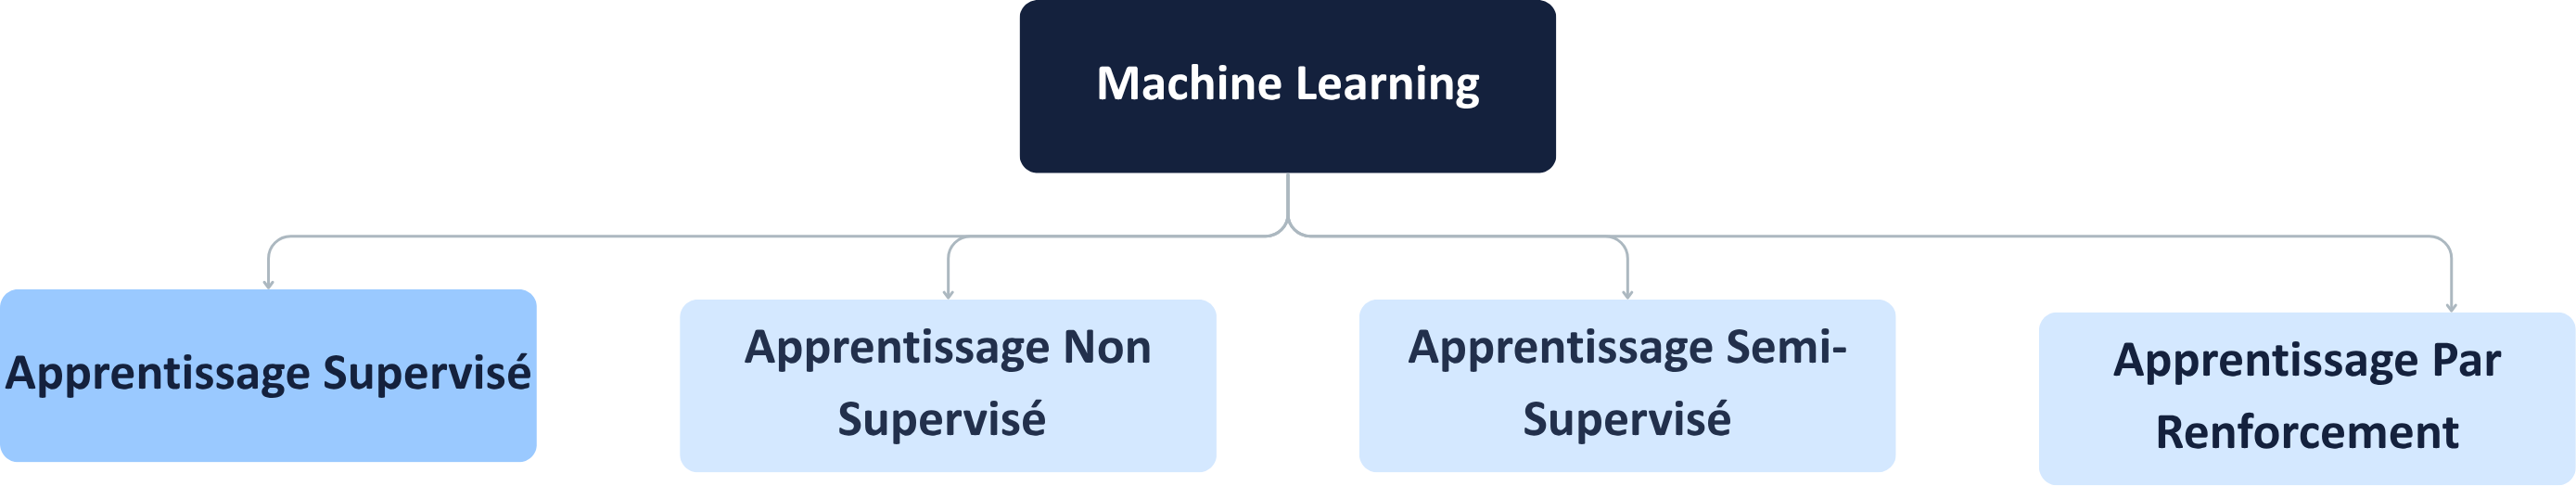
\includegraphics[width=0.85\textwidth]{figures/machinelearningtypes.png}
    \caption{Les quatre familles du Machine Learning.}
    \label{fig:ml-types}
\end{figure}

Dans notre contexte, l'apprentissage \textbf{supervisé} est le seul pertinent~:
nous disposons d'un historique d'exécutions passées (les étiquettes) et l'objectif
est précis : prédire le taux annuel $T4$. Il est important de noter que le ML est
une \textit{branche} de l'intelligence artificielle~: certains systèmes d'IA
fonctionnent par règles écrites manuellement par un expert (on parle de
\textit{systèmes experts}) sans jamais apprendre à partir de données. Dans le
contexte de la prévision budgétaire, où les dynamiques sont trop complexes pour
être encodées à la main, c'est le ML supervisé qui s'impose naturellement.

\paragraph{Le cadre de l'apprentissage supervisé~:}

Dans ce travail, nous utilisons exclusivement l'\textbf{apprentissage supervisé}~: le
modèle apprend à partir d'exemples pour lesquels la «~bonne réponse~» est connue.
Chaque exemple est un couple~:

\begin{itemize}
    \item \textbf{Les variables d'entrée} $\mathbf{x}_i$ (appelées \textit{features})~:
    tout ce qu'on sait \textit{avant} la fin de l'année (taux de réalisation au premier,
    deuxième et troisième trimestre, programme budgétaire, région, part de la ligne dans
    le budget total).
    \item \textbf{La variable à prédire} $y_i$ (appelée \textit{variable cible})~: le
    taux de réalisation annuel final $T4$, connu seulement en fin d'exercice.
\end{itemize}

Le modèle cherche une fonction $f$ telle que $f(\mathbf{x}_i) \approx y_i$~: étant
donné ce qu'on sait en cours d'année, il estime ce que sera le taux final. En termes
formels, l'algorithme minimise une \textbf{fonction de perte} $\mathcal{L}$, qui
mesure l'écart entre la prédiction et la réalité, sur l'ensemble des exemples
historiques~:

$$\hat{f} = \arg\min_{f \in \mathcal{F}} \sum_{i=1}^{n}
\mathcal{L}\bigl(y_i,\, f(\mathbf{x}_i)\bigr)$$

Dans notre application, $\mathcal{L}$ est l'erreur quadratique $(y - \hat{y})^2$, qui
pénalise davantage les grandes erreurs de prédiction.

\paragraph{Comment se déroule un projet de Machine Learning~?}

Un projet de Machine Learning s'inscrit dans un cycle méthodologique structuré, allant
de la collecte des données à leur intégration opérationnelle. Bien que présenté de
manière séquentielle, il convient de souligner d'emblée qu'il s'agit d'un processus
fondamentalement itératif, dans lequel les résultats de chaque phase informent en retour
les décisions prises lors des phases antérieures. Dans le contexte du présent travail,
ce cycle se décline selon les étapes suivantes~:

\begin{enumerate}
    \item \textbf{Collecte des données}~: rassembler des données fiables et
    représentatives. Dans notre cas, il s'agit des rapports trimestriels d'exécution
    budgétaire publiés par la TGR sur la période 2020--2025, complétés par les morasses
    annuelles du ministère de la Justice.
    \item \textbf{Préparation des données}~: nettoyer, structurer et transformer les
    données brutes en un format exploitable par les algorithmes. Cette étape inclut
    la gestion des valeurs manquantes, la création des variables (features) et
    l'encodage des identifiants catégoriels (programme, région).
    \item \textbf{Choix de l'algorithme}~: sélectionner le type de modèle adapté
    au problème. Pour une prévision sur données tabulaires avec historique court,
    Ridge et XGBoost ont été retenus (voir section~3.3).
    \item \textbf{Entraînement du modèle}~: présenter les exemples historiques
    à l'algorithme. Celui-ci ajuste ses paramètres internes pour minimiser l'écart
    entre ses prédictions et les valeurs réelles, selon la formule ci-dessus.
    \item \textbf{Évaluation}~: tester le modèle sur des données qu'il n'a pas
    vues pendant l'entraînement, en mesurant son erreur via le RMSE, le MAE et le
    MAPE. Dans ce travail, cette évaluation se fait par validation walk-forward
    (section~3.4).
    \item \textbf{Amélioration}~: analyser les erreurs commises, ajuster les
    hyperparamètres (profondeur des arbres, taux de régularisation $\lambda$) et
    affiner l'ingénierie des features jusqu'à obtenir des performances satisfaisantes.
    \item \textbf{Déploiement et surveillance}~: intégrer le modèle dans un
    environnement opérationnel et surveiller en continu sa performance sur les
    nouvelles données, en le ré-entraînant si la structure des données évolue.
\end{enumerate}

Ce cycle n'est pas linéaire~: les résultats de l'évaluation conduisent souvent
à revenir sur la préparation des données ou le choix des features. Dans notre
travail, plusieurs itérations ont été nécessaires pour identifier et corriger
les problèmes de fuite de données décrits en section~3.4.

\begin{figure}[h]
    \centering
    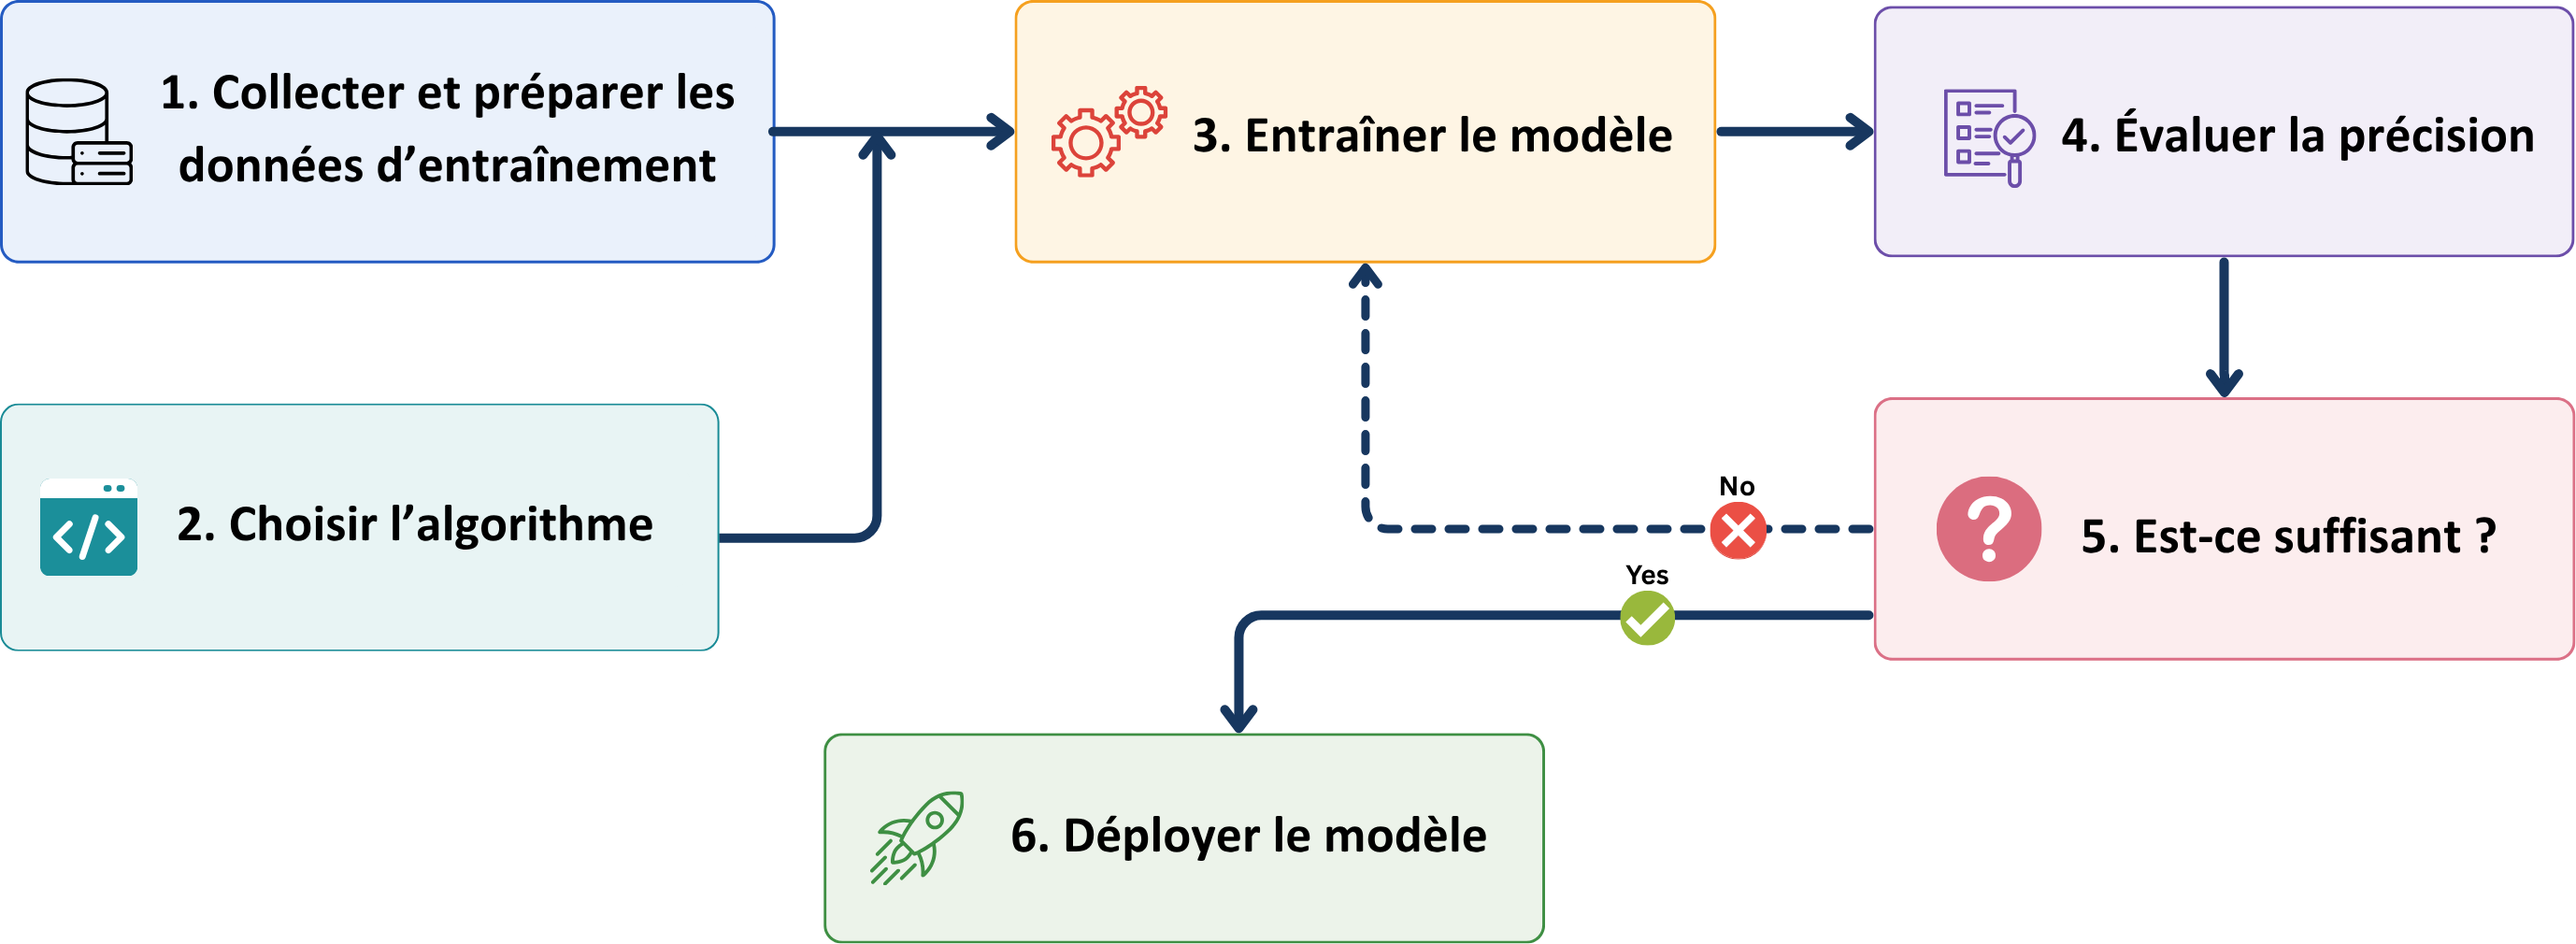
\includegraphics[width=0.85\textwidth]{figures/CommentfonctionneleML.png}
    \caption{Cycle de fonctionnement d'un projet de Machine Learning~: de la
    collecte des données au déploiement, avec itérations d'amélioration.}
    \label{fig:cycle-ml}
\end{figure}

%----------------------------------------------------------------
\phantomsection
\subsubsection*{3.1.2 \quad Pourquoi le Machine Learning}
\addcontentsline{toc}{subsubsection}{3.1.2 Pourquoi le Machine Learning}
%----------------------------------------------------------------

La pr\'evision des taux d'ex\'ecution budg\'etaire pr\'esente trois caract\'eristiques
qui rendent les approches classiques de s\'eries temporelles difficiles \`a appliquer
dans notre contexte~: les comportements sont non lin\'eaires, l'information pertinente
est multidimensionnelle, et l'historique disponible par ligne est court. C'est
pr\'ecis\'ement face \`a ces trois propri\'et\'es que le Machine Learning d\'emontre
le plus clairement sa valeur ajout\'ee.

\paragraph{Non-lin\'earit\'es et effets de seuil~:}

L'ex\'ecution budg\'etaire n'ob\'eit pas \`a une logique de proportionnalit\'e
simple. Une ligne d\'ej\`a \`a 60\,\% de r\'ealisation au deuxi\`eme trimestre
ne se comportera pas du tout de la m\^eme fa\c{c}on qu'une ligne \`a 10\,\%,
m\^eme si l'\'ecart brut avec leur historique respectif est identique. Il existe
des \textbf{effets de seuil et d'acc\'el\'eration}~: au-del\`a d'un certain
niveau d'avancement, la dynamique d'ex\'ecution change de nature. Les algorithmes
ML, en particulier les arbres de d\'ecision (XGBoost), d\'etectent et mod\'elisent
ces ruptures automatiquement, sans qu'on ait besoin de les sp\'ecifier \`a
l'avance.

\paragraph{Int\'egration des variables contextuelles~:}

La capacit\'e d'ex\'ecution d'une ligne budg\'etaire est tributaire d'une multiplicit\'e
de facteurs contextuels~: la cat\'egorie budg\'etaire (Investissement ou Fonctionnement
selon la nature de la d\'epense), le programme de rattachement (Soutien et pilotage,
Performance de l'administration judiciaire, Modernisation du syst\`eme judiciaire et
juridique, ou Renforcement des droits et des libert\'es), la localisation r\'egionale,
la part relative de la ligne dans le budget global, ou encore les profils historiques
de lignes comparables. Les algorithmes ML se distinguent pr\'ecis\'ement par leur capacit\'e
\`a int\'egrer simultan\'ement l'ensemble de ces dimensions et \`a \'etablir, de mani\`ere
automatis\'ee, le poids relatif de chacune d'entre elles selon le type de d\'epense et
l'horizon de pr\'evision consid\'er\'e.

\paragraph{Mutualisation de l'information entre lignes budg\'etaires~:}

Avec seulement 5 \`a 6 ann\'ees d'historique par ligne, tout mod\`ele traitant
chaque ligne s\'epar\'ement travaille sur une base statistique fragile. Le ML
r\'esout ce probl\`eme en \textbf{agr\'egeant toutes les lignes et toutes les
ann\'ees dans un seul jeu d'entra\^inement}~: une ligne qui n'a que 5 ann\'ees
d'historique b\'en\'eficie des patterns observ\'es sur l'ensemble du panel. Le
mod\`ele apprend des r\`egles transversales~: par exemple, que les lignes
d'investissement en retard \`a mi-ann\'ee rattrapent en g\'en\'eral leur d\'eficit
au quatri\`eme trimestre, ou que les lignes de fonctionnement \`a forte part
budg\'etaire sont structurellement pr\'evisibles. Cette mutualisation est l'un
des avantages les plus d\'ecisifs de l'approche dans notre contexte.

\vspace{4pt}
Le tableau suivant synth\'etise ces propri\'et\'es~:

\begin{table}[h]
\centering
\caption{Comparaison des m\'ethodes classiques et des approches de Machine Learning.}
\label{tab:comparaison-ml}
\begin{tabular}{lll}
\hline
\textbf{Propri\'et\'e} & \textbf{M\'ethodes classiques}
& \textbf{ML (Ridge / XGBoost)} \\
\hline
Non-linéarités et effets de seuil & Non & Oui \\
Variables contextuelles multiples & Limité & Naturellement intégrées \\
Courtes séries par ligne & Fragile & Robuste (mutualisation) \\
Interprétabilité & Coefficients & Coefficients (Ridge), importance (XGB) \\
\hline
\end{tabular}
\end{table}

%----------------------------------------------------------------
\phantomsection
\subsubsection*{3.1.3 \quad Limites des approches classiques de prévision}
\addcontentsline{toc}{subsubsection}{3.1.3 Limites des approches classiques de prévision}
%----------------------------------------------------------------

Le chapitre~2 a recensé les principales méthodes de prévision utilisées dans la
littérature budgétaire~: modèles ARIMA/SARIMA, régressions saisonnières, lissages
exponentiels. Ces approches reposent sur des hypothèses qui se révèlent difficiles
à satisfaire dans notre contexte.

Premièrement, elles exigent des séries temporelles suffisamment longues par entité
prédite~: ARIMA recommande au moins 50 observations pour une estimation fiable, ce
qui correspond à plus de 12 années de données trimestrielles par ligne. Avec
seulement 5 à 6 ans d'historique, l'estimation des paramètres est instable et les
intervalles de confiance très larges.

Deuxièmement, ces méthodes traitent chaque ligne budgétaire de façon isolée~: elles
ne peuvent pas exploiter le fait que des lignes relevant du même programme ou de
la même région partagent des dynamiques communes. L'information potentiellement
précieuse contenue dans les centaines de lignes du budget n'est pas mutualisée.

Troisièmement, l'intégration de variables contextuelles explicatives (programme,
région, indicateurs judiciaires) dans un modèle ARIMA requiert des extensions
ARIMAX qui augmentent considérablement sa complexité sans garantir une amélioration
sensible des performances quand l'historique est court. Ces limites motivent le
recours au Machine Learning, dont les apports spécifiques à notre contexte ont été
présentés en section~3.1.2.

%================================================================
\phantomsection
\subsection*{3.2 \quad Apprentissage supervisé}
\addcontentsline{toc}{subsection}{3.2 Apprentissage supervisé}
%================================================================

%----------------------------------------------------------------
\phantomsection
\subsubsection*{3.2.1 \quad Généralisation}
\addcontentsline{toc}{subsubsection}{3.2.1 Généralisation}
%----------------------------------------------------------------

Un modèle ML n'a de valeur que s'il prédit correctement des situations qu'il n'a
\textit{jamais vues}. Or un algorithme suffisamment puissant peut «~mémoriser~»
tous ses exemples d'entraînement sans réellement comprendre les patterns sous-jacents.
Ce phénomène s'appelle le \textbf{surapprentissage} (\textit{overfitting})~: le
modèle performe brillamment sur ses données d'entraînement et échoue sur de
nouvelles données. La \textbf{généralisation} désigne précisément la capacité d'un
modèle à maintenir ses performances sur des données inédites, critère
déterminant pour un usage opérationnel.

La généralisation dépend d'un équilibre délicat entre la complexité du modèle et
la quantité de données disponibles. Un modèle trop simple ne captera pas les
patterns importants~; un modèle trop complexe les mémorisera sans les comprendre.
Cet équilibre est formalisé par le compromis biais-variance.

%----------------------------------------------------------------
\phantomsection
\subsubsection*{3.2.2 \quad Le compromis biais-variance}
\addcontentsline{toc}{subsubsection}{3.2.2 Le compromis biais-variance}
%----------------------------------------------------------------

L'erreur totale d'un modèle peut toujours se décomposer en trois termes~:

$$\text{Erreur totale} = \underbrace{\text{Biais}^2}_{\text{modèle trop simple}}
+ \underbrace{\text{Variance}}_{\text{modèle trop complexe}}
+ \text{Bruit irréductible}$$

\begin{itemize}
    \item Le \textbf{biais} traduit un \textit{sous-apprentissage}~: le modèle est
    trop simple et rate des patterns importants. Exemple~: supposer que le taux final
    est toujours égal au taux du deuxième trimestre.
    \item La \textbf{variance} traduit un \textit{surapprentissage}~: le modèle est
    trop complexe et apprend le bruit au lieu du signal. Il s'adapte parfaitement à
    l'historique, mais généralise mal.
    \item Le \textbf{bruit irréductible}~: une partie de la réalité est par nature
    imprévisible (décisions politiques de dernière minute, suspensions de dépenses
    imprévues, événements exceptionnels). Aucun modèle ne peut l'éliminer.
\end{itemize}

Les métriques d'évaluation quantifient cet écart entre prédictions et réalité.
Trois indicateurs sont utilisés dans ce travail~:

$$\text{RMSE} = \sqrt{\frac{1}{n}\sum_{i=1}^{n}(y_i - \hat{y}_i)^2} \qquad
\text{MAE} = \frac{1}{n}\sum_{i=1}^{n}|y_i - \hat{y}_i| \qquad
\text{MAPE} = \frac{100}{n}\sum_{i=1}^{n}\left|\frac{y_i - \hat{y}_i}{y_i}\right|\,\%$$

\begin{itemize}
    \item Le \textbf{RMSE} (Racine de l'Erreur Quadratique Moyenne) est la métrique
    principale. Il pénalise plus fortement les grandes erreurs~: se tromper de 20\,\%
    est bien pire que deux erreurs de 10\,\%.
    \item Le \textbf{MAE} (Erreur Absolue Moyenne) donne l'erreur typique en valeur
    absolue, moins sensible aux cas exceptionnels.
    \item Le \textbf{MAPE} (Erreur Absolue Moyenne en Pourcentage) exprime l'erreur
    en pourcentage, ce qui facilite la comparaison entre lignes de niveaux très
    différents.
\end{itemize}

Dans notre protocole, le RMSE sert de critère principal de sélection des modèles~;
MAE et MAPE sont présentés en complément dans les tableaux du chapitre~4.

%----------------------------------------------------------------
\phantomsection
\subsubsection*{3.2.3 \quad Surapprentissage et robustesse}
\addcontentsline{toc}{subsubsection}{3.2.3 Surapprentissage et robustesse}
%----------------------------------------------------------------

Avec seulement 5 à 6 années d'historique par ligne, un modèle très complexe risque
fortement de mémoriser les données plutôt que d'en extraire des règles généralisables.
Nous privilégions donc des modèles \textbf{régularisés} (Lasso et XGBoost avec
pénalités $L_1/L_2$) qui incluent un mécanisme interne limitant leur propre
complexité, trouvant ainsi le bon équilibre entre simplicité et précision.

Trois contraintes spécifiques à notre contexte plafonnent par ailleurs la précision
atteignable~:

\begin{enumerate}
    \item \textbf{Volume de données limité}~: cinq à six années d'historique par ligne
    représentent un volume modeste. Les modèles à grand nombre de paramètres risquent
    de mémoriser ces quelques exemples plutôt que d'en extraire des règles robustes.

    \item \textbf{Données partiellement synthétiques}~: les taux d'exécution publiés
    par la Trésorerie Générale du Royaume (TGR) sont des agrégats par catégorie, sans
    ventilation par programme ni par région. La construction du panel désagrégé repose
    donc sur une simulation calibrée (décrite au chapitre~4), ce qui introduit une
    imprécision structurelle dans les données d'entraînement.

    \item \textbf{Variables non observables}~: certains facteurs qui influencent
    l'exécution budgétaire ne figurent tout simplement pas dans les données : une
    décision de suspendre temporairement des dépenses en cours d'année, un retard
    dans le lancement d'un appel d'offres, ou une réallocation de crédits d'un
    programme vers un autre décidée au niveau central. Ces événements, invisibles
    pour le modèle, peuvent pourtant modifier significativement le niveau de
    consommation observé en fin d'année. Même le meilleur algorithme ne peut pas
    prédire ce qu'il ne voit pas.
\end{enumerate}

%================================================================
\phantomsection
\subsection*{3.3 \quad Les modèles retenus}
\addcontentsline{toc}{subsection}{3.3 Les modèles retenus}
%================================================================

Quatre modèles ont été évalués dans ce travail~: deux \textbf{benchmarks naïfs}
(sans apprentissage statistique) qui servent de barre minimale, et deux
\textbf{algorithmes ML} à proprement parler. Le choix a été guidé par deux critères~:
la pertinence théorique face aux données budgétaires, et la faisabilité d'un
déploiement réel dans une administration publique (un modèle trop opaque ou trop
coûteux à maintenir n'a pas de valeur opérationnelle).

%----------------------------------------------------------------
\phantomsection
\subsubsection*{3.3.1 \quad Modèles de référence (benchmarks naïfs)}
\addcontentsline{toc}{subsubsection}{3.3.1 Modèles de référence (benchmarks naïfs)}
%----------------------------------------------------------------

Avant l'introduction de tout modèle sophistiqué, il convient d'établir des références
méthodologiques simples~: des prévisions qu'un gestionnaire pourrait produire sans recours
à des techniques avancées, et qui constituent dès lors la borne minimale que tout modèle
de Machine Learning se doit de surpasser pour justifier sa complexité additionnelle.

\paragraph{Benchmark 1~: Moyenne historique~:}

Le benchmark le plus élémentaire repose sur l'extrapolation directe de la performance
historique~: si une ligne a réalisé en moyenne 82\,\% de son enveloppe annuelle au cours
des cinq derniers exercices, on projette ce même taux d'exécution pour l'année en cours.

$$\hat{y}_i = \frac{1}{N} \sum_{t=1}^{N} y_{i,t}$$

\noindent\small\textit{où $\hat{y}_i$ est la prévision pour la ligne $i$, $N$ le nombre d'années d'entraînement, et $y_{i,t}$ le taux d'exécution réel de la ligne $i$ en année $t$.}\normalsize

Ce benchmark capture la \textbf{persistance structurelle} du taux d'exécution~:
certaines lignes sont structurellement bien exécutées, d'autres chroniquement
sous-exécutées. Ignorer cet historique serait une erreur.

\paragraph{Benchmark 2~: Naïf saisonnier lag-4~:}

Une variante alternative consiste à projeter, pour l'année courante, le taux d'exécution
exactement réalisé lors de l'exercice antérieur.

$$\hat{y}_i = y_{i,\, Y-1}$$

\noindent\small\textit{où $y_{i,\, Y-1}$ est le taux d'exécution réel de la ligne $i$ l'année précédente.}\normalsize

Ce benchmark s'avère souvent difficile à surpasser en pratique, dans la mesure où il
capture implicitement les phénomènes d'inertie institutionnelle et les tendances récentes
de la dynamique budgétaire. Par conséquent, un modèle de Machine Learning incapable de
produire des prévisions plus fiables que cette simple reconduction n'apporte aucune
valeur ajoutée opérationnelle.

Ces deux benchmarks constituent la \textbf{barre minimale} que les modèles ML doivent
franchir pour justifier leur déploiement.

%----------------------------------------------------------------
\phantomsection
\subsubsection*{3.3.2 \quad Ridge (régularisation)}
\addcontentsline{toc}{subsubsection}{3.3.2 Ridge (régularisation)}
%----------------------------------------------------------------

\paragraph{Principe en langage clair~:}

La régression linéaire classique cherche la combinaison de variables qui prédit le
mieux le taux final~: «~le taux final vaut approximativement $a$ fois le taux T2,
plus $b$ fois la part budgétaire, plus une constante~». Le problème~: avec beaucoup
de variables et peu d'observations, le modèle peut attribuer des coefficients
aberrants à des variables peu informatives, ce qui nuit à la généralisation.

Le \textbf{Ridge} (Tikhonov regularization) ajoute une contrainte~: les coefficients
trop grands sont pénalisés. Contrairement au Lasso qui force certains coefficients
à zéro, Ridge réduit progressivement tous les coefficients vers zéro sans les
éliminer complètement. Cela produit un modèle plus stable et robuste, particulièrement
utile en présence de données avec outliers.

$$\min_{\beta_1,\ldots,\beta_p} \;\; \underbrace{\frac{1}{n}\sum_{i=1}^{n}(y_i - \hat{y}_i)^2}_{\text{erreur de prédiction}} \;+\; \lambda \underbrace{\sum_{j=1}^{p}\beta_j^2}_{\text{pénalité L2 sur les coefficients}}$$

\noindent\small\textit{Les $\beta_j$ sont les coefficients du modèle. $\lambda$ est choisi par validation croisée.}\normalsize

Le paramètre $\lambda$ contrôle l'intensité de cette contrainte~: plus $\lambda$ est
grand, plus les coefficients sont réduits. Sa valeur est choisie automatiquement par
validation croisée (voir section~3.4).

\paragraph{Pourquoi Ridge pour les dépenses de matériel~?}

Les dépenses de matériel et dépenses diverses ont un profil d'exécution
\textbf{régulier et prévisible}, avec peu de variation d'une année à l'autre. Dans
ce contexte, l'hypothèse de linéarité est raisonnable. Ridge est particulièrement
adapté car (1) il limite le surapprentissage sur peu de données, (2) il conserve
tous les prédicteurs même faibles, ce qui améliore la stabilité face aux outliers,
et (3) ses résultats restent interprétables~: un gestionnaire peut comprendre qu'
«~une hausse d'un point de pourcentage du taux au deuxième trimestre se traduit par
une hausse de $\beta_{T2}$ points du taux annuel final~».

\textbf{Note sur la normalisation~:} Les variables d'entrée doivent être normalisées avant
d'être soumises à Ridge. Deux stratégies sont possibles~: le \textit{StandardScaler},
fondé sur la moyenne et l'écart-type (optimal pour distributions gaussiennes, sensible
aux valeurs extrêmes), ou le \textit{RobustScaler}, fondé sur la médiane et l'intervalle
interquartile (plus robuste en présence d'outliers). Le choix dépend de la structure
des données. Dans ce travail, le \textit{RobustScaler} s'est révélé supérieur sur
les dépenses de matériel car il neutralise les anomalies de courte durée (voir
section 4.5.5 pour les détails d'optimisation post-validation).

%----------------------------------------------------------------
\phantomsection
\subsubsection*{3.3.3 \quad Méthodes d'ensemble (XGBoost)}
\addcontentsline{toc}{subsubsection}{3.3.3 Méthodes d'ensemble (XGBoost)}
%----------------------------------------------------------------

\paragraph{Principe en langage clair~:}

Le \textbf{gradient boosting} repose sur un principe de correction itérative des erreurs
mis en œuvre par un ensemble séquentiel de modèles faibles~: un premier modèle produit
une estimation initiale~; chaque modèle subséquent se concentre spécifiquement sur la
correction des résidus engendrés par les précédents. Cette approche cumulative, par laquelle
l'ensemble des corrections successives s'agrègent, conduit à une prévision globale
sensiblement plus fidèle que celle qu'aurait pu fournir un modèle unique considéré
isolément.

Dans XGBoost, chaque «~expert~» est un \textbf{arbre de décision}~: une suite de
questions simples du type «~est-ce que le taux T2 est supérieur à 45\,\%~?~» qui
débouche sur une prévision. L'algorithme construit une séquence d'arbres
$T_1, T_2, \ldots, T_K$, chacun corrigeant les erreurs du précédent~:

$$\underbrace{\hat{y}_i^{(k)}}_{\text{nouvelle pr\'evision}} = \underbrace{\hat{y}_i^{(k-1)}}_{\text{pr\'evision pr\'ec\'edente}} + \eta \cdot \underbrace{T_k(x_i)}_{\text{correction de l'arbre }k}$$

où $\eta$ est un «~taux d'apprentissage~» qui contrôle à quel point chaque correctif
est appliqué (une valeur faible rend l'apprentissage plus prudent). La prévision
finale est la somme de tous les arbres~:

$$\hat{y}_i = \sum_{k=1}^{K} \eta \cdot T_k(x_i)$$

Pour éviter le surapprentissage, chaque arbre est contraint dans sa complexité par
des paramètres de régularisation~: limite sur la profondeur des arbres, pénalités
sur les feuilles, et sous-échantillonnage aléatoire des données à chaque étape.

\paragraph{Pourquoi XGBoost pour les dépenses d'investissement~?}

Le choix de XGBoost pour les dépenses d'investissement se fonde sur une observation
empirique déterminante~: les dynamiques d'exécution de cette catégorie présentent des
\textbf{non-linéarités prononcées}. À titre d'illustration, une ligne dont le taux
d'exécution s'établit à 5\,\% au deuxième trimestre, rattachée à un programme
d'investissement en infrastructure, peut atteindre 80\,\% en clôture d'exercice grâce
à des décaissements massifs concentrés en fin d'année --- phénomène qu'un modèle
linéaire ne saurait anticiper. XGBoost s'avère particulièrement adapté à ce type de
configuration, et ce pour les raisons suivantes~:

\begin{itemize}
    \item Il capture naturellement les \textbf{effets de seuil et les interactions}~:
    l'effet du taux T2 peut être différent selon le programme, la région ou la taille
    de la ligne.
    \item Il \textbf{généralise bien avec peu de données}~: contrairement aux réseaux
    de neurones, XGBoost est efficace avec quelques centaines d'observations grâce à
    sa régularisation intégrée.
    \item Il est \textbf{interprétable}~: l'importance de chaque variable (combien elle
    contribue en moyenne aux prédictions) peut être extraite et présentée à des
    gestionnaires non-spécialistes.
    \item Il est \textbf{open-source et rapide}~: déployable sans licence commerciale,
    son exécution sur un ordinateur de bureau standard prend quelques secondes,
    un impératif dans un contexte ministériel.
\end{itemize}

%----------------------------------------------------------------
\phantomsection
\subsubsection*{3.3.4 \quad Couche de détection d'anomalies}
\addcontentsline{toc}{subsubsection}{3.3.4 Couche de détection d'anomalies}
%----------------------------------------------------------------

En complément des prévisions, le système intègre une \textbf{couche de détection
d'anomalies de sous-exécution}. Le principe est simple~: \textit{le système calcule
un score Z par ligne, comparant son taux d'exécution T2 à sa propre moyenne
historique. Une déviation de plus de 1,5~écarts-types déclenche une alerte
opérationnelle.} Formellement, pour chaque ligne budgétaire $i$, on calcule un
\textbf{score Z} comme suit~:

$$z_i = \frac{\text{taux}_{i,\text{T2}} - \mu_i}{\sigma_i}$$

\noindent\small\textit{où $\mu_i$ et $\sigma_i$ sont la moyenne et l'écart-type du
taux T2 de la ligne $i$ sur les années d'entraînement.}\normalsize

Une ligne est \textbf{signalée comme anomalie} si $z_i < -1{,}5$, ce qui indique
que son niveau d'exécution à mi-année est statistiquement anormal par rapport à
son propre historique. Trois niveaux de sévérité sont distingués~:

\begin{itemize}
    \item \textbf{Exécution nulle}~: taux T2~$= 0$, aucun décaissement enregistré~;
    \item \textbf{Sous-exécution sévère}~: $z_i < -2$, écart très inhabituel~;
    \item \textbf{Sous-exécution modérée}~: $-2 \leq z_i < -1{,}5$, signal d'alerte préventive.
\end{itemize}

Cette couche ne constitue \textit{pas} une détection de fraude au sens pénal~: elle
identifie des \textbf{anomalies opérationnelles} -- lignes bloquées administrativement,
crédits non encore délégués, ou projets n'ayant pas démarré -- qui nécessitent une
intervention de pilotage avant la clôture de l'exercice.

%----------------------------------------------------------------
\phantomsection
\subsubsection*{3.3.5 \quad Justification des modèles écartés}
\addcontentsline{toc}{subsubsection}{3.3.5 Justification des modèles écartés}
%----------------------------------------------------------------

\paragraph{Principe~:}

Le Random Forest fonctionne lui aussi sur le principe d'une «~équipe d'arbres~»,
mais différemment~: au lieu de travailler en séquence (chacun corrigeant le
précédent), les arbres travaillent \textbf{en parallèle et indépendamment}, chacun
entraîné sur un sous-ensemble aléatoire des données. La prévision finale est la
moyenne de toutes leurs réponses~:

$$\hat{y}_i = \frac{1}{B} \sum_{b=1}^{B} \underbrace{T_b(x_i)}_{\text{r\'eponse de l'arbre }b}$$

\noindent\small\textit{$B$ arbres votent ind\'ependamment~; la pr\'evision finale est leur moyenne.}\normalsize

Cette indépendance réduit le risque de surapprentissage, mais elle a un coût~: les
arbres ne se corrigent pas mutuellement, ce qui les rend moins précis individuellement.

\paragraph{Pourquoi Lasso a été écarté~:}

Lasso (Least Absolute Shrinkage and Selection Operator) a initialement été considéré
pour prédire les dépenses de matériel, car il offre une sélection automatique des
prédicteurs. Cependant, la validation walk-forward a révélé ses limitations~:

\begin{enumerate}
    \item \textbf{Sensibilité aux outliers}~: Le mécanisme de sélection (force
    certains coefficients à zéro) peut ètre fragilisé par quelques valeurs extrêmes,
    conduisant à des modèles instables d'une année à l'autre.
    \item \textbf{Ridge plus stable}~: Ridge (Régularisation L2) réduit progressivement
    tous les coefficients sans les éliminer, produisant une meilleure stabilité
    face aux outliers par normalisation avec RobustScaler.
    \item \textbf{Performance empirique}~: Sur les données du ministère de la Justice,
    Ridge + RobustScaler a surpassé Lasso + StandardScaler de 9,1~points de RMSE
    (voir section 4.5.5).
\end{enumerate}

Lasso est néanmoins documenté dans les tableaux de comparaison du chapitre~4 comme
algorithme initialement testé ; sa évaluation comparative appuie la pertinence du
choix de Ridge pour ce contexte.

\paragraph{Pourquoi Random Forest a été écarté~:}

Random Forest a été évalué lors de la validation walk-forward (détaillée au
chapitre~4), mais n'a pas été retenu comme modèle de production, pour trois raisons~:

\begin{enumerate}
    \item \textbf{Performances inférieures}~: XGBoost a systématiquement produit des
    erreurs plus faibles sur les dépenses d'investissement, la catégorie la plus
    complexe. L'entraînement sur des sous-échantillons aléatoires peut éliminer
    des patterns utiles quand les données sont rares.
    \item \textbf{Incapacité à extrapoler}~: les arbres de décision ne peuvent pas
    prédire au-delà des valeurs observées pendant l'entraînement. Pour des lignes
    dont les taux 2025 dépassent tous les niveaux historiques, Random Forest plafonne
    méchaniquement, tandis que XGBoost peut s'ajuster prudemment.
    \item \textbf{Parcimonie opérationnelle}~: dans un contexte de déploiement réel,
    retenir le modèle le plus performant par catégorie est préférable à empiler
    plusieurs algorithmes dans un ensemble hybride difficile à expliquer et à maintenir.
\end{enumerate}

Random Forest est néanmoins présenté dans les tableaux de résultats du chapitre~4
comme point de comparaison ; sa mise en concurrence avec les autres modèles est un
élément de rigueur méthodologique essentiel.

%================================================================
\phantomsection
\subsection*{3.4 \quad La validation rigoureuse}
\addcontentsline{toc}{subsection}{3.4 La validation rigoureuse}
%================================================================

Construire un modèle ML n'est que la moitié du travail. L'autre moitié consiste à
\textbf{mesurer honnêtement sa performance}~: combien d'erreur fait-il sur des
données qu'il n'a jamais vues~? Cette question semble simple, mais elle cache un
piège redoutable dans le contexte des séries temporelles.

%----------------------------------------------------------------
\phantomsection
\subsubsection*{3.4.1 \quad Les données temporelles}
\addcontentsline{toc}{subsubsection}{3.4.1 Les données temporelles}
%----------------------------------------------------------------

\paragraph{La validation croisée standard~: efficace mais inadaptée ici~:}

La validation croisée en $k$ groupes (\textit{k-fold}) constitue la méthode standard
d'évaluation des modèles de Machine Learning~: l'ensemble des données est partitionné
en $k$ sous-ensembles disjoints~; à chaque itération, l'un de ces sous-ensembles est
réservé au test, tandis que le modèle est entraîné sur les $k-1$ sous-ensembles
restants. La performance globale est alors estimée par la moyenne des erreurs sur
l'ensemble des folds.

\begin{table}[h]
\centering
\caption{Sch\'ema de la validation crois\'ee $k$-fold (exemple~: Groupe~2 = test).}
\label{tab:kfold}
\begin{tabular}{|c|c|c|c|c|}
\hline
\textbf{Groupe 1} & \cellcolor{primary!40}\textbf{Groupe 2} & \textbf{Groupe 3} & \textbf{Groupe 4} & \textbf{Groupe 5} \\
\hline
Entr. & \textbf{Test} & Entr. & Entr. & Entr. \\
\hline
\end{tabular}\\[4pt]
{\scriptsize Groupe 2 = test~; groupes 1, 3, 4, 5 = entra\^inement}
\end{table}

Si cette approche demeure valide lorsque les observations satisfont l'hypothèse
d'indépendance mutuelle, son application à des données temporelles introduit un biais
méthodologique critique~: la permutation aléatoire des années au sein des groupes de
validation autorise le modèle à accéder, lors de son entraînement, à des informations
postérieures à la période qu'il est censé prédire. Autrement dit, un modèle ayant
«~observé~» les réalisations de 2024 pour prédire celles de 2022 bénéficie d'une
divulgation implicite d'information temporelle, ce qui invalide dès lors la mesure de
sa capacité prédictive réelle.

\paragraph{La contrainte fondamentale~: toujours prédire vers l'avant~:}

Pour les séries temporelles, une règle doit être respectée absolument~: les données
d'entraînement doivent toujours être antérieures aux données de test. Cela donne
naissance à des protocoles de validation spécifiques.

%----------------------------------------------------------------
\phantomsection
\subsubsection*{3.4.2 \quad Validation walk-forward}
\addcontentsline{toc}{subsubsection}{3.4.2 Validation walk-forward}
%----------------------------------------------------------------

Le protocole retenu dans ce travail est la \textbf{validation walk-forward à fenêtre
expansive}, qui reproduit fidèlement le cadre opérationnel auquel se trouvera confronté
le décideur en conditions réelles. Concrètement~:

\begin{itemize}
    \item Pour prédire l'année 2022, le modèle s'entraîne uniquement sur 2020--2021.
    \item Pour prédire 2023, il s'entraîne sur 2020--2022.
    \item Pour prédire 2024, il s'entraîne sur 2020--2023.
    \item Pour prédire 2025, il s'entraîne sur 2020--2024.
\end{itemize}

La caractéristique centrale de cette approche réside dans l'élargissement progressif
de la fenêtre d'entraînement à chaque étape temporelle, reflétant l'accumulation
naturelle d'expérience historique au fil du temps. Ainsi, plus l'horizon de prévision
se rapproche du présent, plus le modèle bénéficie d'un volume substantiel de données
antérieures. La performance globale est in fine estimée en moyennant les erreurs commises
sur les quatre périodes de test ainsi définies.

\begin{table}[h]
\centering
\setlength{\tabcolsep}{4pt}
\caption{Protocole de validation walk-forward \`a fen\^etre expansive (2022--2025).}
\label{tab:walkforward}
\begin{tabular}{l|ccccc}
\hline
 & \textbf{2021} & \textbf{2022} & \textbf{2023} & \textbf{2024} & \textbf{2025} \\
\hline
Fold 1 (test 2022) & \cellcolor{accent!30}Entr. & \cellcolor{primary!40}\textbf{Test} & & & \\
Fold 2 (test 2023) & \cellcolor{accent!30}Entr. & \cellcolor{accent!30}Entr. & \cellcolor{primary!40}\textbf{Test} & & \\
Fold 3 (test 2024) & \cellcolor{accent!30}Entr. & \cellcolor{accent!30}Entr. & \cellcolor{accent!30}Entr. & \cellcolor{primary!40}\textbf{Test} & \\
Fold 4 (test 2025) & \cellcolor{accent!30}Entr. & \cellcolor{accent!30}Entr. & \cellcolor{accent!30}Entr. & \cellcolor{accent!30}Entr. & \cellcolor{primary!40}\textbf{Test} \\
\hline
\end{tabular}\\[4pt]
{\scriptsize \colorbox{accent!30}{\strut Entra\^inement} \quad
\colorbox{primary!40}{\strut Test} \quad Cases vides = donn\'ees non encore disponibles}
\end{table}

Ce protocole présente trois avantages majeurs~:

\begin{itemize}
    \item \textbf{Simulation exacte du déploiement réel}~: chaque fold reproduit
    fidèlement la situation du gestionnaire : il dispose de tout l'historique passé
    et prédit l'année courante.
    \item \textbf{Aucune contamination temporelle}~: à aucun moment le modèle n'est
    entraîné sur des données postérieures à l'année qu'il prédit.
    \item \textbf{Mesure de la progression}~: comparer les erreurs du fold 2022 (peu
    de données) à celles du fold 2025 (plus de données) quantifie l'apport de chaque
    année d'historique supplémentaire.
\end{itemize}

%----------------------------------------------------------------
\phantomsection
\subsubsection*{3.4.3 \quad Risque de data leakage}
\addcontentsline{toc}{subsubsection}{3.4.3 Risque de data leakage}
%----------------------------------------------------------------

\paragraph{Qu'est-ce que la fuite de données~?}

La \textbf{fuite de données} (\textit{data leakage}) est une erreur qui consiste à
laisser entrer dans le processus d'entraînement des informations qui ne seraient pas
disponibles au moment d'une vraie prévision. Le modèle apprend alors des patterns
«~trop faciles~» qui disparaissent en production. Le symptôme est trompeur~: les
métriques de validation semblent excellentes, mais le modèle déçoit une fois déployé.

\paragraph{Mécanisme 1~: fuite par le protocole de validation~:}

Si le jeu de test est l'année~2022 mais que le modèle s'entraîne sur des données
incluant 2023, 2024 et 2025, il «~voit l'avenir~» pendant l'entraînement. La méthode
LOYO (\textit{Leave-One-Year-Out}) commet exactement cette erreur~: pour tester 2022,
elle entraîne sur toutes les autres années y compris les années ultérieures, ce qui
produit des métriques artificiellement optimistes. Le walk-forward élimine ce risque
par construction.

\paragraph{Mécanisme 2~: fuite par les variables explicatives~:}

Même avec un bon protocole, la fuite peut s'introduire lors de la construction des
variables. Exemple typique~: si on calcule «~la moyenne historique des taux T3 de
cette ligne sur toutes les années disponibles~» et qu'on l'utilise pour prédire 2022,
cette moyenne inclut les années 2023, 2024, 2025, soit des données futures. La solution
est de calculer cette moyenne de façon \textbf{causale}~: pour prédire l'année $Y$,
n'utiliser que les années strictement antérieures à $Y$.

%----------------------------------------------------------------
\phantomsection
\subsubsection*{3.4.4 \quad Prévision directe vs roulante}
\addcontentsline{toc}{subsubsection}{3.4.4 Prévision directe vs roulante}
%----------------------------------------------------------------

\paragraph{Motivation pratique~:}

La validation walk-forward présentée en section~3.4.2 garantit une séparation temporelle
stricte~: le modèle ne voit jamais d'information future. Cependant, cette approche
reflète un scénario académique où l'on prédisait à~$t=0$ l'intégralité d'une année
budgétaire sans aucune donnée intra-annuelle.

En réalité, les gestionnaires budgétaires ne prédisent pas deux ans à l'avance~: ils
ont besoin de réviser les prévisions en cours d'exécution. Par exemple, à la mi-année
(T2 écoulé), on dispose déjà des taux d'exécution réels pour T1 et T2, et l'enjeu est
de prédire le taux final T4. Cette situation est fondamentalement différente, car elle
combine~:
\begin{enumerate}
  \item Une \textbf{fenêtre d'observation}~: données passées réelles (T1, T2)
  \item Une \textbf{fenêtre de prédiction}~: données futures inconnues (T4)
  \item Une \textbf{fenêtre intermédiaire}~: T3, potentiellement prédite ou observée
\end{enumerate}

\paragraph{Deux stratégies de prédiction~:}

\textbf{Approche directe~:} Le modèle reçoit directement T1 et T2 observés comme entrées
et produit en un seul passage la prédiction de T4 finale. Cette approche suppose que la
relation $(T1, T2) \to T4$ peut être apprise directement depuis les données historiques,
sans étape intermédiaire.

\textbf{Approche roulante~:} Le processus de prédiction se décompose en deux étapes
séquentielles~:
\begin{enumerate}
  \item \textbf{Étape 1~:} Prédire T3 à partir de T1 et T2 observés
  \item \textbf{Étape 2~:} Prédire T4 à partir de T1, T2 observés \textit{et} T3 prédit
\end{enumerate}

L'approche roulante capture une structure temporelle progressive~: on suppose que T3 est
informatif pour prédire T4, et que les modèles bénéficient de cette information
intermédiaire, même si elle est elle-même entachée d'erreur de prédiction.

\paragraph{Implications méthodologiques~:}

Cette distinction revêt une importance capitale pour la conception du système de
prévision. Alors que la validation walk-forward teste la capacité du modèle à
généraliser dans le temps, la comparaison directe vs roulante interroge la
\textbf{structure causale} de la prédiction~: faut-il modéliser la dépendance
$(T1, T2) \to T4$ de façon monolithique, ou la décomposer en étapes qui reflètent le
déroulement temporel réel du trimestre~?

Les deux stratégies restent dans le cadre de la validation walk-forward~: aucune
information de T4 (année de test) ne fuit dans l'entraînement. Cependant, elles
interrogent comment \textit{structurer} la prédiction lorsqu'on dispose d'information
partielle en cours d'année. Cette question présente un caractère à la fois théorique
(quelle est la meilleure approche conceptuellement~?) et pratique (laquelle produit
des prévisions plus fiables en situation opérationnelle~?). Les résultats empiriques
figurent au chapitre~4.

%----------------------------------------------------------------
\phantomsection
\subsubsection*{3.4.5 \quad Évaluation des modèles}
\addcontentsline{toc}{subsubsection}{3.4.5 Évaluation des modèles}
%----------------------------------------------------------------

Le taux de réalisation au troisième trimestre ($T3$, disponible fin septembre) est
un prédicteur très puissant du taux annuel final. Mais si le modèle est utilisé
\textit{en juin} (après T2), inclure T3 constituerait une fuite~: cette information
n'existe pas encore. Notre implémentation propose donc deux prévisions distinctes~:
\begin{itemize}
    \item une \textbf{prévision du T4 basée sur T2}, disponible en juin (sans T3)~;
    \item une \textbf{prévision du T4 basée sur T3}, disponible en octobre (avec T3).
\end{itemize}

Cette distinction illustre que la maîtrise de la fuite de données est avant tout une
condition de \textbf{confiance opérationnelle}~: un modèle qui triche en entraînement
produira des alertes erronées en production. Les détails d'implémentation sont
présentés au chapitre~4.

%================================================================
\phantomsection
\subsection*{3.5 \quad Synthèse du chapitre}
\addcontentsline{toc}{subsection}{3.5 Synthèse du chapitre}
%================================================================

Ce chapitre a établi les fondements sur lesquels repose la démarche empirique
du mémoire. Le Machine Learning a été justifié face aux approches classiques par sa
capacité à mutualiser l'information entre lignes, à capturer des non-linéarités, et
à fonctionner avec peu d'historique individuel. Parmi les quatre modèles évalués,
Ridge et XGBoost ont été retenus pour leurs performances et leur adéquation au
contexte opérationnel~; Lasso et Random Forest ont été évalués mais écartés. Enfin,
la validation walk-forward (section~3.4.2) a été présentée comme le seul protocole
qui simule fidèlement les conditions de déploiement réel, en éliminant par
construction tout risque de fuite temporelle. Une variante pratique a également été
proposée (section~3.4.4)~: la prévision \textit{directe} vs \textit{roulante}, qui
capture deux stratégies de prédiction selon que le gestionnaire dispose déjà de
l'observation de T3 ou non.

Le chapitre suivant décrit la mise en œuvre empirique de ces principes~: construction
des données, implémentation des folds walk-forward, et résultats comparatifs obtenus
sur le périmètre du ministère de la Justice pour la période 2022--2025.
